\chapter{Introdução}\label{cap:introducao}

Sistemas de Segmentação de Imagem tem se tornado populares em variadas
aplicações, desde a área de edição de imagem, diagnósticos médicos e
parte da visão computacional necessária pra reconhecimento de
objetos. Entre estes motivos e outros, esta área tem uma relevância
científica alta considerando a situação social, tecnológica e
econômica que é vivida no século XXI.\@

\begin{figure}[h!]
        \captionsetup{width=16cm}
		\Caption{\label{fig:image-segmentation-types}
          Comparação de tipos de segmentação de imagem: por semântica
          e instância}
		\centering
		\UFCfig{}{
			\fbox{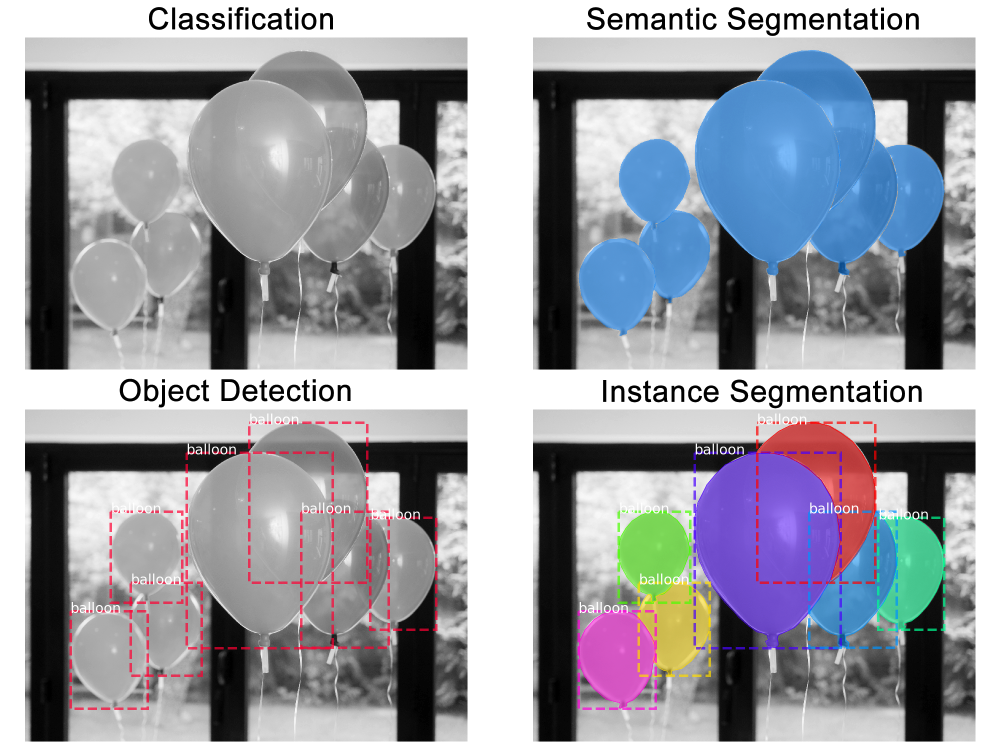
\includegraphics[width=16cm]{figuras/image-segmentation-types}}
		}{
			\Fonte{\citeonline{MediumInstanceSegmentation2019}}
		}
\end{figure}


Segmentação de Imagens podem ser feitas manualmente por um anotador
humano marcando as linhas delineadoras de um objeto em foco na
imagem. Por outro lado, é conhecido algoritmos variados para
segmentação de imagens baseado em aprendizagem de máquina. Entre as
abordagens com aprendizagem, é selecionado neste trabalho
especificamente a aprendizagem semi-supervisionada.


Considerando a dificuldade de conseguir dados anotados feito por
humanos em ambientes de uso especialistas, como imagens médicas e
ferramentas de edição de imagem, a abordagem semi-supervisionada se
demonstra interessante por necessitar poucos dados anotados, mas ainda
existir anotação com viés do especialista interessado (médico,
editor).

Os três principais algoritmos clássicos de segmentação de imagem podem
ser citados: \textit{Region-Based Segmentation}; \textit{Edge Detection
  Segmentation}; \textit{Segmentation based on Clustering}
\cite{ImageSegmentationTechniques1985}. Cada uma dessas técnicas
possuem limitações conhecidas, entre elas é possível mencionar: ter
muitos objetos na imagem podem dificultar a segmentação, tempo
computacional elevado, sensível ao contraste em escala cinza.

A abordagem estado da arte atual para segmentação de imagem utiliza
\textit{Convolutional Neural Networks} (CNN), a técnica é conhecida
como \textit{Mask R-CNN} \cite{he2018mask}, funciona bem em casos
diversos e supera as técnicas anteriores nas métricas de segmentação,
mas possui ainda uma grande limitação: alto custo computacional para
treinamento da rede neural profunda e muitos dados anotados são necessários.

Considerando tal situação-problema, este trabalho será conduzido sobre
a construção de uma técnica de segmentação de imagem
semi-supervisionada utilizando redes complexas e dinâmicas coletivas
de tal maneira que tenha menor complexidade computacional em relação a
\textit{Mask R-CNN} e seja robusto sobre os problemas enfrentados pelas
técnicas clássicas.
